\section{Face authentication}
    Brief introduction to the section.

    \subsection{Data set}
    We have set requirements for our dataset, aiming to reflect real-life
    appliances:
    \begin{itemize}
        \item \textbf{depth and IR channels}: in real-life appliance, leveraging
        the infrared camera allows equally good vision regardless of lighting
        conditions.
        \item \textbf{various vertical angles}: when a user is looking at their
        mobile device,
        their head may be placed at various angles along the vertical axis.
        However, it is reasonable to assume that the angle along the horizontal
        axis will be small, especially if the user is consciously trying to
        unlock the device.
        \item \textbf{many frames per subject}: when a new user is being added
        to a mobile device's authentication system, it is acceptable to require
        them to look at the camera, at various angles, for a short period of
        time. Many frames can (and should) be taken.
    \end{itemize}

    There are several good databases for face recognition with depth camera:
    The EURECOM Kinect Face Database\cite{eurecom},
    RGB-D Face database \cite{vapaaudk},
    The Florence Superface dataset\cite{superface}. However, none of them was
    deemed suiting for our project, primarily due to the lack of IR channel.
    Thus, we have decided to build a dedicated dataset.

    \subsubsection*{Data collection}
    The dataset consists of \textbf{TODO} subjects: \textbf{TODO} males and
    \textbf{TODO} females, mostly aged $20$-$25$. Each subject has been asked to
    follow an object with their entire head, making two cycles of slow,
    continuous movements: \texttt{up $\to$ center $\to$ down $\to$ center $\to$
    left $\to$ center $\to$ right $\to$ center}.
    That procedure has resulted in approximately $20$ seconds of footage per
    subject.

    IR and depth frames are synchronized, taken at $10$ FPS rate.

    Dataset contains also RGB frames taken at $10$ FPS rate, not synchronized
    with IR and depth frames.

    \subsubsection*{Test set}
    \textbf{TODO: update if that changes}
    For the test set, we have chosen approximately first $25\%$ of
    frames from each subject -- the first two vertical head rotations.

    \subsubsection*{Samples}
    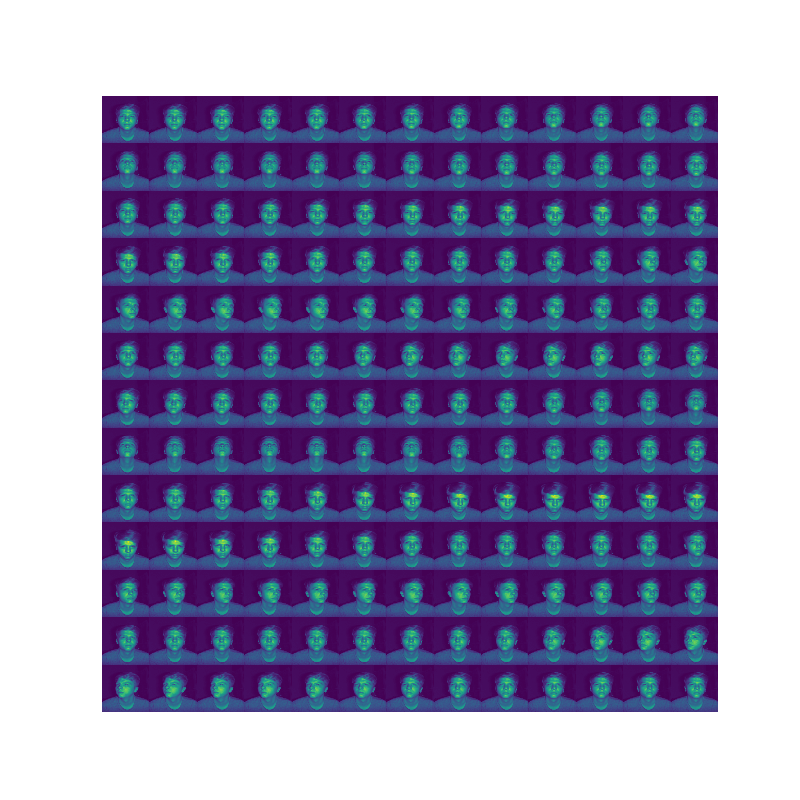
\includegraphics[scale=0.5]{tiled_faces_3}

    \subsection{Face angle detection}
    Longer description of angle detection

    \subsection{Normalization}
        \subsubsection*{Mean and std. dev. normalization}
        Dropping corner values, chosen mean and std. dev. values.

        \subsubsection*{Face angle normalization}
        Use of face angle detection to rotate to frontal position.
        \textbf{TODO 3d plots}

    \subsection{Preprocessing techniques}
    We have tried several different preprocessing techniques.
        \subsubsection*{Trimming faces}
        During the process of collecting the dataset, each subject has been
        recorded in only one set of clothes (the ones they were wearing at the
        time), one hairstyle and the background may slightly vary among the
        subjects (the background behind subjects recorded at $12$ a.m. is
        likely to be brighter than behind the subjects recorded at $4$ p.m.).

        Since a classifier might leverage those factors, photos have been
        trimmed to polygons containing the faces. Such polygons have been
        found with Face Recognition library \cite{facerecog} on IR photos.
        Depth photos have been trimmed accordingly.
        \textbf{TODO image samples}

        \subsubsection*{Entropy maps}
        How they work, why to use them (reference to the other paper).

        \subsubsection*{HOGs of entropy maps}
        How they work, why to use them (reference to the other paper). They
        are particularly helpful for Extra Trees and RDF-s.

        \subsubsection*{Skin mask channel}
        Link to some section from skin-recognition about how it is calculated.
        Short description and motivation that it may make sense for
        convolutions.
        Sample photos.

        \subsubsection*{Channels vs concatenation}
        A choice of the input format passed to a classifier is not only a matter
        of images to include. Another decision to be made is whether different
        channels (IR, depth) and different preprocessed images (entropy maps,
        HOGs) should be concatenated or layered as channels. In our experiments,
        we have included both approaches.


    \subsection{Classifiers}
        \subsubsection*{CNN}

        \subsubsection*{Voting SVMs and Extra Trees}

        \subsubsection*{Voting CNN, SVMs and Extra Trees}

    \subsection{Quality measures}
        \subsubsection*{ACC}

        \subsubsection*{AUC ROC}

        \subsubsection*{Recall for fixed precision}


    \subsection{Test results}
        \begin{tabular}{ |c|c|c|c|c|c|c|c|c|c|c|c|c| }
            \hline
            \multirow{2}{*}{Model} &
            \multirow{2}{*}{Mode} &
            \multirow{2}{*}{Trim} &
            \multirow{2}{*}{Rotation} &
            \multirow{2}{*}{Entropy} &
            \multirow{2}{*}{HOGs} &
            \multirow{2}{*}{Skin mask} &
            \multirow{2}{*}{Inputs} &
            \multirow{2}{*}{ACC} &
            \multirow{2}{*}{AUC ROC} &
            \multicolumn{3}{|c|}{Recall for precision $\rho$} \\
            & & & & & & & & & & $\rho = 0.99$ & $\rho = 0.995$ & $\rho = 0.999$ \\
            \hline
            CNN & binary & polygon & frontal & y & y & n & channels & NA & 0.86 & 0.9 & 0.85 & 0.83 \\
            \hline
        \end{tabular}
